\documentclass{article}
\usepackage[margin=.5in]{geometry}
\usepackage{graphicx, dblfloatfix}
\usepackage{amsmath, amssymb, amsfonts, mathrsfs, mathtools, physics}
\usepackage{gensymb}
\usepackage[english]{babel}
\usepackage[autostyle, english = american]{csquotes}
\usepackage[normalem]{ulem}
\usepackage[title,titletoc,toc]{appendix}
\usepackage{pgfplotstable}
\usepackage{array, booktabs, colortbl, caption}
\usepackage{braket}
\MakeOuterQuote{"}

\newcommand{\redchi}{$\tilde{\chi}^2\,$}
\renewcommand{\vec}[1]{\mathbf{#1}}

\title{Parity of Positronium}
\author{Alejandro Legarda}

\begin{document}
\raggedright
\maketitle

\begin{abstract}
We investigate the photons produced in para-positronium decay to confirm the conservation of parity through the decay. We expect, due to conservation of parity, that two identical photons will be emitted by the decay in orthogonally plane-polarized configurations. We use this and the fact that photons preferentially scatter in the direction orthogonal to their plane polarization during Compton scattering to show evidence of odd parity in the two-photon system, and hence conservation of parity for the decay process.
\end{abstract}
	
	
\tableofcontents
\newpage

\section{Theory}

Positronium is a "meta-stable particle" composed of an electron and a positron in a bound state. When positronium decays by annihilation, two or three photons, depending on the initial spin-states, will be emitted. We are interested in the decay into two photons, which is the preferred decay channel of para-positronium, which has a total spin s = 0. We know already, then, that spin will be conserved in this decay. The photons, by conservation laws, must be identical, and are emitted simultaneously. Due to conservation of parity, the two photons will be preferentially plane-polarized orthogonal to one another. By measuring the correlation of the two photon polarizations, the conservation of parity in electromagnetic interactions can be tested.

\hspace{.25cm}

Parity is a conserved quantity in electromagnetic interactions. Both para- and ortho-positronium have odd parity before the decay; therefore, the parity of the system after the decay should also be odd. The wave-function for a two photon state with momenta $\vec{k}$ and $\vec{-k}$, and photon frequency $\omega$, and exhibiting odd parity can be show to be proportional to

\begin{equation}
	[\braket{|\hat{\epsilon_1}}\braket{|\hat{\epsilon_2}} - \braket{|\hat{\epsilon_2}} \braket{|\hat{\epsilon_1}}] \cross [exp(i (\vec{k} \cdot \vec{r} - 2\omega t)) - exp(i (- \vec{k} \cdot \vec{r} - 2\omega t))]
\end{equation}

where $\vec{r = r_1 - r_2}$, and $\hat{\epsilon_1}$, $\hat{\epsilon_2}$ are the photon polarizations. The expectation for this wavefunction is at a maximum when the planes of polarization are orthogonal. We therefore expect to observe a greater number of photon pairs with orthogonal polarizations than pairs with parallel polarizations.

\hspace{.25cm}

We can take advantage of this preferential polarization to test parity conservation. We use an aluminum scatterer to "catch" the emitted photons. Aluminum has a low enough density that we will expect exactly one instance of Compton scattering per photon. The photons enter the aluminum rod and scatter out without interacting again before reaching a detector. The angle at which the photon is scattered from the aluminum is dependent on the polarization. This is evidenced in the Klein-Nishina formula,

\begin{figure}[!htb]
	\centering
	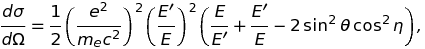
\includegraphics[scale=.5]{eqn_6.png}
 	\label{klein}
\end{figure}

where $\frac{d\sigma}{d\Omega}$ is the differential cross section, e is the electron charge and $\eta$ is the angle between the incident photon polarization and the scattering plane. In our geometry $\theta \approx$  90$\degree$, so the cross section is maximized when $\eta$ = 90$\degree$ or 270$\degree$. That is, the cross section for scattering is highest when the plane of scattering is perpendicular to the plane of polarization.

\section{Method}
\subsection{Apparatus}

\begin{figure}[!htb]
	\centering
	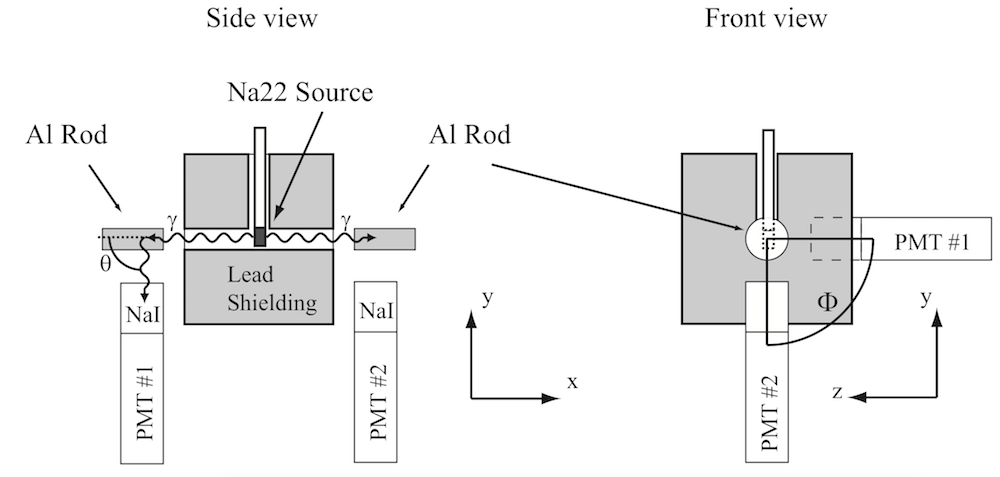
\includegraphics[scale=.5]{apparatus.png}
  	\caption{The experimental apparatus. A Na-22 source is housed inside lead shielding. Aluminum rods are aligned with the openings of the shielding, which Compton scatter photons into the photomultiplier tubes.}
	\caption{Refer to bib item [1]}
 	\label{Apparatus}
\end{figure}

The setup consists primarily of a Na-22 source with two opposite openings in its shielding, allowing for photons to exit in opposite directions. Aligned with these opening, we have aluminum scatterers, that will do the be Compton scattering the photons at an angle dependent on their polarization. We then have two photomultiplier tubes that rotate 360$\degree$ around the rods. We will be positioning these at 90$\degree$ intervals, starting at 45$\degree$ to the horizontal. The setup therefore allows us to test every perpendicular and parallel configuration for the PMTs.

The apparatus operates as follows: Once a photon enters a PMT, the PMT will provide a pulse to describe the photon it detected. Any pulses that are not large enough to have been cause by a 90$\degree$ Compton-scattered gamma photon are rejected. This helps to get rid of a lot of background noise. The discriminator output pulses go into a second discriminator, and the outputs from the second discriminator go into one channel of a coincidence unit. This coincidence unit produces an output pulse only when it reads two pulses, one from each PMT, within 50 ns from each other. This output goes to a scaler.
A second set of outputs from the second-level discriminator, with the pulse from the second PMT delayed by 100 ns, goes to a second channel of the coincidence unit.[1]

\hspace{.25cm}

Every time a signal is measured in one PMT within 50 ns to a signal from the other is counted as a coincidence, and a scaler is incremented by one. The second scaler is incremented each time a pulse from one PMT is coincident with a delayed pulse from the other. We choose a 100 ns delay such that any coincidences recorded on the second scalar are not true, but random. This represents the background rate of accidental coincidences.

\hspace{.25cm}

\subsection{Accidental Coincidence Rate}

In theory, we can approximate the number of accidental coincidences by using the following formula

\begin{gather}
	R_{acc} = R_1 R_2 \tau \\
	\tau = w_1 + w_2 - 2w_0
\end{gather}

where $w_1, w_2$ are the widths of the two discriminator output pulses, and were $w_0$ is the minimum overlap required to fire the coincidence unit. We find that predicted coincidence rates from calculation agree with the values calculated by the apparatus. The correct coincidence rate can therefore be calculated by subtracting the coincidence rate measured in the second scaler from the coincidence rate from the first scaler.

\section{Analysis}


\begin{table}[]
\centering
\caption{Singles and Coincidence Rates}
\label{table}
\begin{tabular}{@{}llllllllll@{}}
\toprule
Angle1 & Angle2 & Count Rate1 & Count Rate2 & Coinc. Ct. & ACC & Coinc. Rate & ACR         & Expctd. ACR & CR error    \\ \midrule
315    & 315    & 381  & 1040  & 96         & 5             & 0.303 & 0.017 & 0.0182     & 0.0327 \\
45     & 315    & 481  & 928  & 133        & 6             & 0.423 & 0.02        & 0.0205     & 0.038 \\
135    & 315    & 480  & 1040  & 128        & 10            & 0.393 & 0.0333 & 0.0230     & 0.0377 \\
225    & 315    & 479  & 1100  & 119        & 5             & 0.380        & 0.0167 & 0.0241     & 0.0364 \\
225    & 45     & 428      & 1105  & 109        & 5             & 0.347 & 0.0167 & 0.0218     & 0.0348 \\
225    & 135    & 441  & 1100  & 147        & 7             & 0.467 & 0.0233 & 0.0224     & 0.0404 \\
225    & 225    & 497  & 1020  & 9         & 3             & 0.290        & 0.010        & 0.0234     & 0.0316 \\
135    & 225    & 490  & 940       & 158        & 6             & 0.507 & 0.020        & 0.0212     & 0.0419  \\
45     & 225    & 480  & 890 & 113        & 8             & 0.350        & 0.0267 & 0.0198     & 0.0354 \\
315    & 225    & 487  & 967  & 131        & 12            & 0.397 & 0.040        & 0.0217     & 0.0382 \\
315    & 135    & 459  & 1010      & 128        & 7             & 0.403 & 0.0233 & 0.0212     & 0.0377 \\
315    & 45     & 425          & 1010  & 154        & 6             & 0.493 & 0.020        & 0.0197     & 0.0414 \\
135    & 45     & 429  & 986  & 177        & 6             & 0.570        & 0.020        & 0.0194     & 0.0443 \\
45     & 45     & 427       & 938.  & 151        & 10            & 0.470        & 0.0333 & 0.0184     & 0.0410 \\
45     & 135    & 456  & 953  & 242        & 5             & 0.790        & 0.0167 & 0.0200     & 0.0519 \\
135    & 135    & 458       & 995  & 151        & 7             & 0.480        & 0.0233 & 0.0209     & 0.0410 \\ \bottomrule
\end{tabular}
\end{table}

Table 1 contains all the data in the form of count rates that the apparatus collects. The runs were each 300 seconds long. In this table, CR stands for Coincidence Rate and ACR stands for Accidental Coincidence Rate. The error in the coincidence rate is calculated using the typical square root model for counting errors. We can see that the uncertainties n this are rather large, on the order of 10\%. From looking at the table, one can see that the accidental rate calculated by the apparatus agrees well with the expected (calculated) accidental count rate (within $2\sigma$).

\hspace{.25cm}

The asymmetry ratio is equal to the ratio of coincidence rate in perpendicular configuration against the coincidence in parallel configuration. By averaging perpendicular and parallel data separately, and propagating uncertainties, we calculate the asymmetry ratio to be

\begin{equation}
	R_{asymmetry} = 1.3 \pm 0.2.
\end{equation}

Where the uncertainty comes from uncertainty in the coincidence rates as a square-root counting error. They were propagated using fractional uncertainties:

\begin{gather}
	\delta_{asymmetry} = [\frac{\delta_{perpendicular}}{R_{perpendicular}} + \frac{\delta_{parallel}}{R_{parallel}}] \cross R_{asymmetry} \\
	R_{perpendicular} = \frac{\Sigma R_i}{N/2}; N=16 \\
	\delta_{perpendicular} = \Sigma \frac{\delta_i}{R_i} \cross R_{perpendicular} \\
	R_{parallel} = \frac{\Sigma R_j}{N/2} \\
	\delta_{parallel} = \Sigma \frac{\delta_j}{R_j} \cross R_{parallel}
\end{gather}

\hspace{.25cm}

Where i corresponds to perpendicular PMT setups and j to parallel setups.
Our experimental setup had values of $\theta = 40\degree, \phi = 30\degree$. From the following graph (Figure 3) we can determine that this corresponds to an asymmetry ratio of about $1.35 \pm 0.05$. This falls in agreement of $1\sigma$ with our calculated value.

\begin{figure}[!htb]
	\centering
	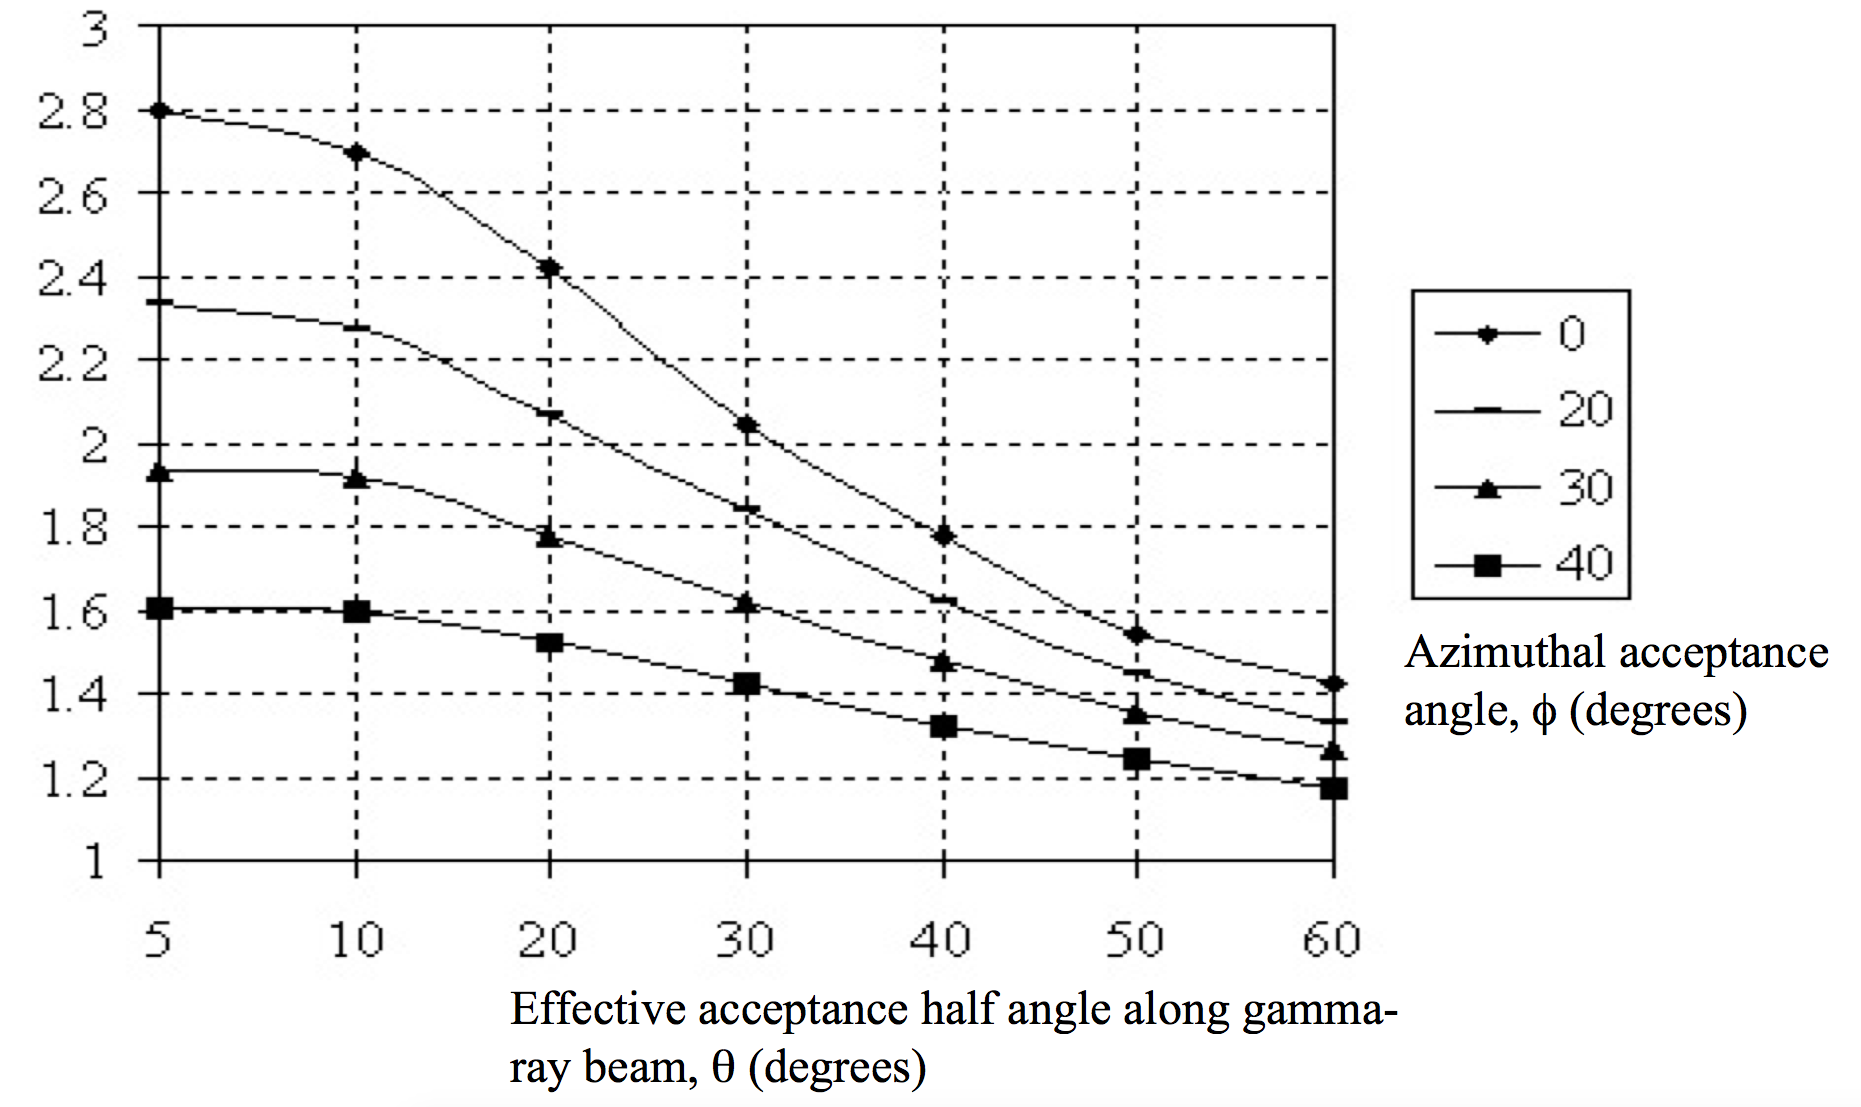
\includegraphics[scale=.2]{Fig_6.png}
 	\label{graph}
	\caption{Refer to bib item [1]}
\end{figure}

\newpage

\section{Conclusion}

We conclude that our data shows conservation of parity for positronium decay, in that is shows an asymmetry ratio that is statistically above 1. As explained in the introduction, this would imply preferential plane-polarization perpendicular between the two decay photons.

\hspace{.25cm}

The most significant source of uncertainty in our experiment was due to the need to readjust the apparatus. Towards the end of the data collection - for the last four or five data points - the apparatus had been manually realigned (by me) because in changing the PMT angles it had come out of alignment. Surprisingly, it turned out that when I aligned the apparatus it ended up better aligned than before, and as such counts were higher overall. This is why some of the late parallel data points are actually higher than some of the lowest perpendicular data points. This resulted in a lower asymmetry ratio than we would have expected. It is important, if one is to repeat this experiment, to maintain the setup as static as possible. This is difficult, as we are required to alter the setup to carry on with the experiment. It would be useful if the apparatus was more firmly fixed. Otherwise, the uncertainty came from unavoidable counting error.


\begin{thebibliography}{10}

	\bibitem{lab manual}
		University of Chicago Department of Physics. "Parity of Positronium"\\
		https://wiki.uchicago.edu/display/P211manuals/Parity+Of+Positronium. (Accessed Apr, 2016)

	\bibitem{taylor}
		Taylor, John. \emph{An Introduction to Error Analysis}. Sausalito: University Science Books, 1997.
		
\end{thebibliography}

\end{document}